
\section{Introducción}

%%Aquí se describe la metodología
%Introducir en términos generales en que consiste la metodología del proyecto, explicar cada paso de manera breve sin recurrir a tantos detalles (términos generales)%
Como parte de la metodología del presente trabajo de investigación se enlistan los pasos mostrados en la figura \ref{fig_0_met}, la idea general del proyecto es dado un par de capturas con zonas enfocadas y desenfocada, se procede a realizar el filtrado de las zonas desenfocadas, esto permitió dejar únicamente las zonas enfocadas en la imagen que posteriormente serán segmentadas, obteniendo así diferentes objetos en cada cuadro, cada uno de los objetos fue caracterizado con la finalidad de poder realizar un seguimiento con respecto al cuadro anterior, finalmente se recupera la profundidad de campo para poder realizar el modelado tridimensional a partir de las zonas enfocadas. 
Este proceso se realiza de manera repetitiva de tal forma que se compara el cuadro actual con el cuadro anterior.

\begin{figure}
\centering
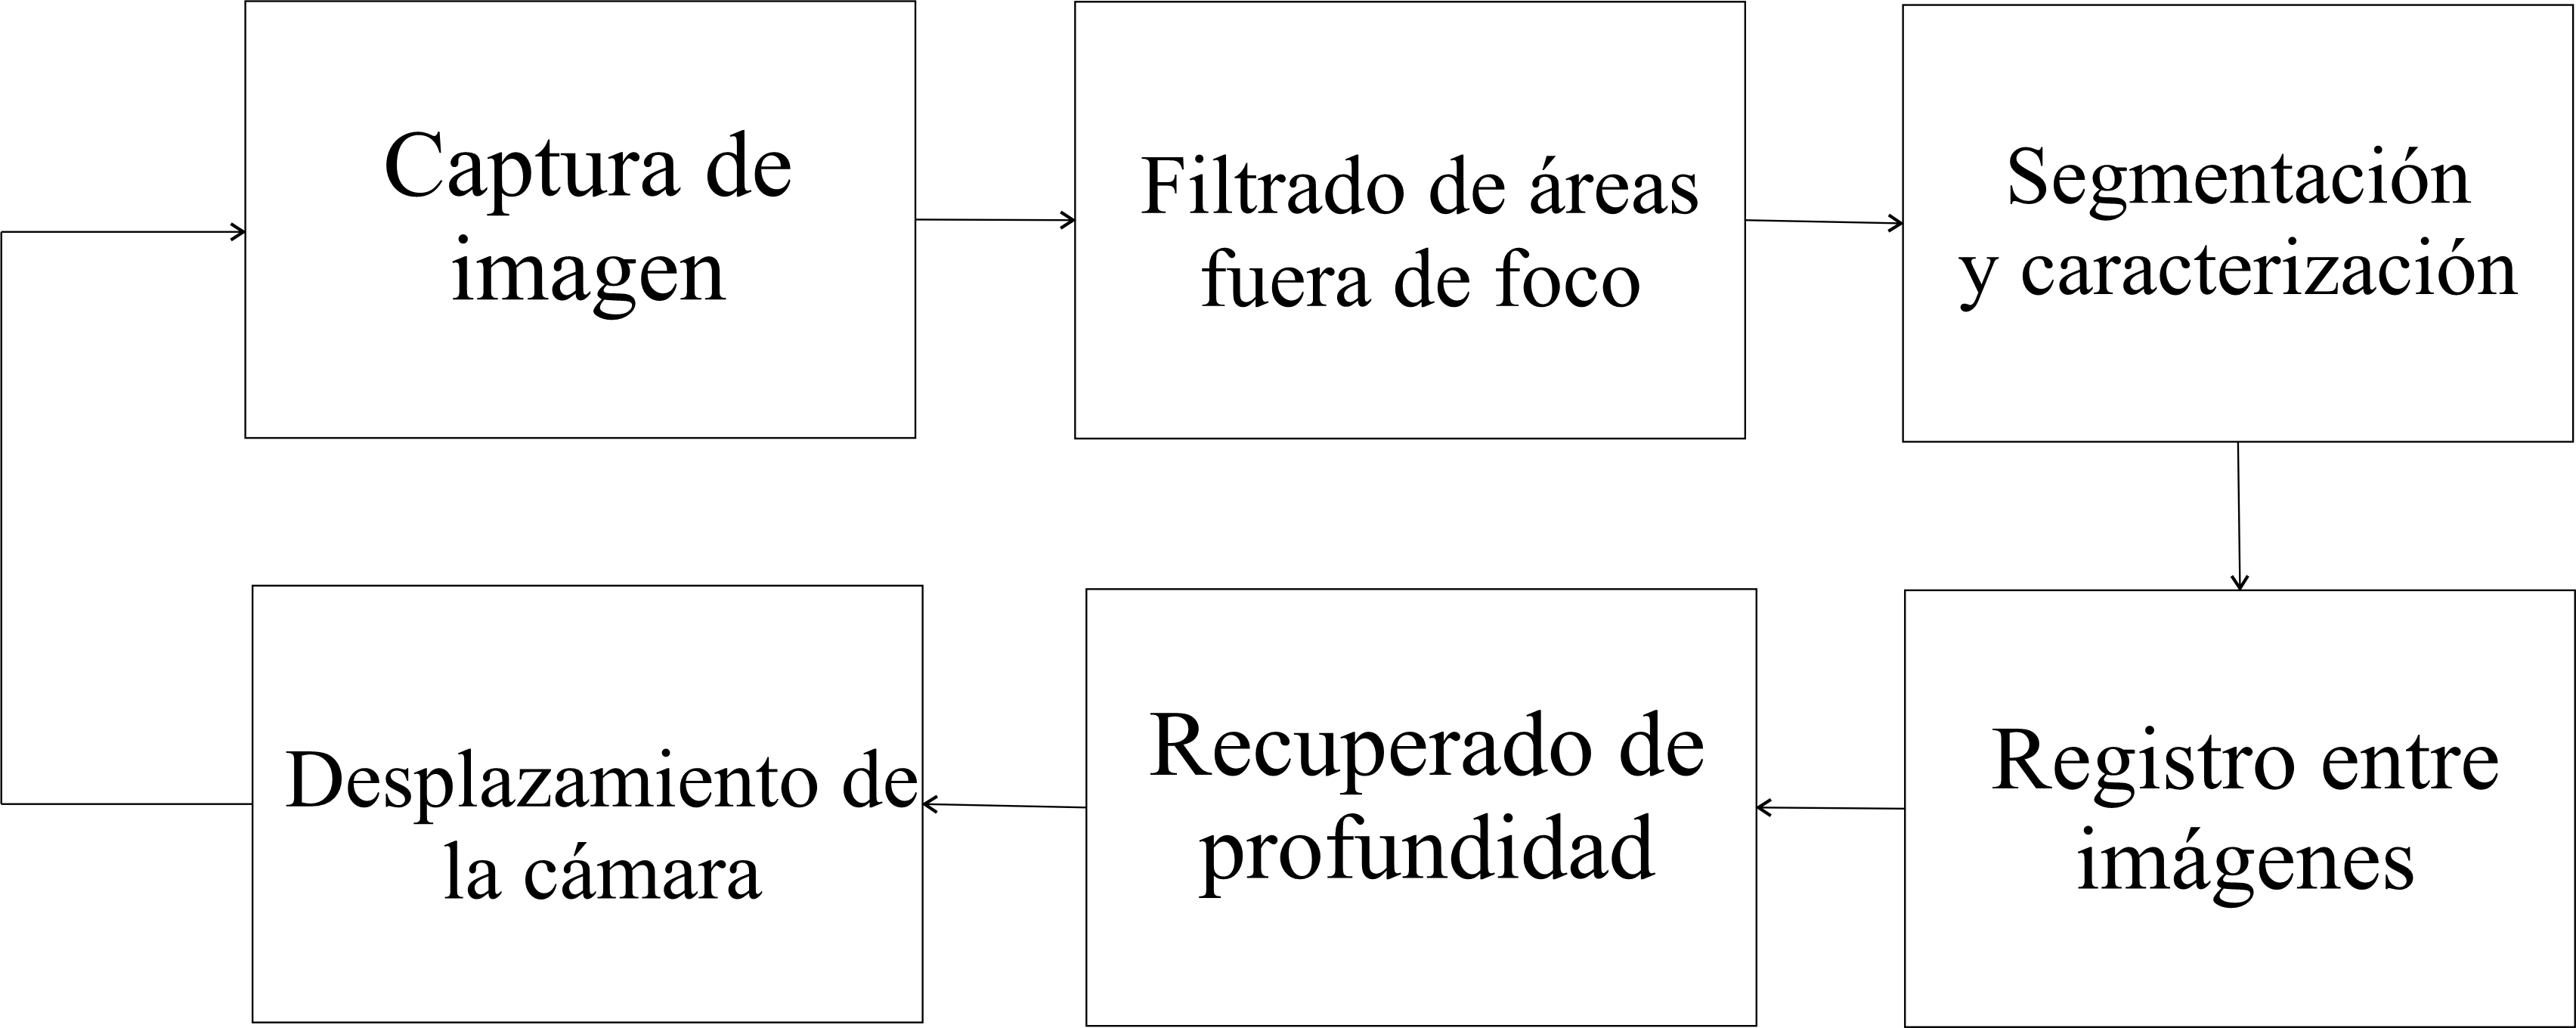
\includegraphics[scale=0.5]{GraficosMetodologia/MetodologiaGeneral.png} 
\caption{Pasos a seguir para el desarrollo general del proyecto}
\label{fig_0_met}
\end{figure}

%Posteriormente realizar la conexión entre la explicación general y la explicación específica por cada uno de los pasos.

A continuación se presentan cada uno de los pasos explicados de manera detallada:



\section{Captura de imagen}

\begin{figure}
\centering
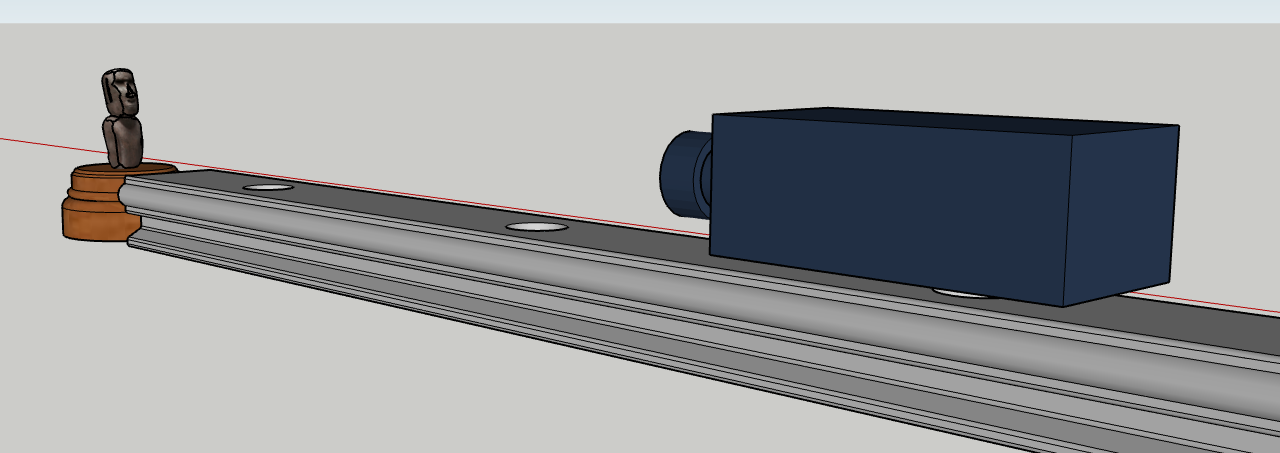
\includegraphics[scale=0.30]{GraficosMetodologia/CapturaDeImagen.png} 
\caption{Modelo de montaje de la cámara sobre la riel.}
\label{modelCapturaImagen}
\end{figure}
El proceso de captura de imagen consta de una cámara montada sobre una riel, la cámara se encuentra dirigida hacia un objeto y esta se desplaza hacia adelante y hacia atrás, de tal forma que se genera una imagen con diferente profundidad de campo de acuerdo a la distancia al objeto \citet{Zhang:14}, en la figura \ref{modelCapturaImagen} se realizó el montaje utilizando un programa de modelado tridimensional con la finalidad de tener una mejor visualización de lo explicado con anterioridad.

%Mencionar cuales materiales se utilizarán en este apartado
%Mencionar las características de la cámara, y el montaje de ella sobre la riel.
%Mencionar el tipo de lente utilizado

\section{Filtrado de áreas desenfocadas}

%Mencionar el método a utilzar para poder eliminar areas fuera de foco
%Argumentar porque ese método es elegido.

%Mostrar algún esquemático que incluya el diseño de este apartado.

%Argumentar porqué se hizo cada cosa.
%Explicar la sálida esperada de este apartado. 
\section{Segmentación y caracterización}
Tras obtener la salida de la imagen en el paso previo se requirió realizar un proceso de segmentado, dicho proceso se encuentra conformado por una umbralización y hallar los contornos, para dar lugar a los objetos de las zonas enfocadas de la imagen original.
\subsection{Umbralización}
Aplicar el proceso de umbralización ayuda a obtener una mejor definición de las zonas enfocadas con las desenfocadas, ya que al aplicar el método de filtrado, resulta que existen zonas desenfocadas que no fueron filtradas por el método, entonces el pre-procesamiento de binarización ayuda a poder eliminar esas zonas que no son de interés.\\
Como pre-procesamiento opcional, también se procede a aplicar el operador de dilatación, esto dependerá del objeto capturado.

\subsection{Búsqueda de contornos}
    Hallar los contornos no solamente ayuda para poder representar visualmente las zonas enfocadas como una máscara, sino también son necesarias para poder realizar una caracterización de los objetos, que posteriormente serán utilizados.\\
\\
Entre las características que fueron de utilidad para este trabajo de investigación se encuentran: los momentos y momentos de Hu.
\subsection{Momentos y Momentos de Hu}
    En \citet{Flusser2009} se mencionan a los momentos invariantes que nos permiten definir cantidades inmutables para cada objeto, dada una rotación, traslación y escalamiento. En particular se hace uso del área del objeto y el centro de masa, que permite definir un conjunto correspondencias entre cada par de capturas.

\section{Registro entre imágenes}
%Mencionar sobre el seguimiento de objetos mencionados por el autor 
La finalidad de este apartado es obtener un método que realice un seguimiento de múltiples objetos por mediante sus centros de masa. Teniendo en cuenta que cada cuadro capturado por medio del desplazamiento de la cámara, dicho desplazamiento puede ser hacia adelante o hacia atrás, lo que ocasiona un escalamiento del objeto, por lo tanto el método tiene que ser robusto para poder despreciar el escalamiento y asociar cada objeto con su respectivo en la captura previa o siguiente. 
\subsection{Correspondencias}
Se establecieron correspondencias entre cada uno de los cuadros, asociando objetos de acuerdo a su distancia euclideana mínima (equación \ref{euclideaneqn}), un proceso similar al algoritmo del vecino más cercano mencionado en el capítulo 4 de \citet{Waltz2008}, el algoritmo compara su distancia entre cada par de objetos (del cuadro actual y el anterior) y establece correspondencias de acuerdo a los emparejamientos resultantes a las distancias mínimas.
\begin{equation}
d = \sqrt{(x_f-x_i)^2 +(y_f - y_i)^2} 
\label{euclideaneqn}
\end{equation}
\subsection{Punto de fuga}
Previo a la búsqueda del punto de fuga, se generó una secuencia de imágenes con la finalidad de poder..... 
En la implementación actual se encontraron hileras de correspondencias, que posteriormente fueron mapeadas a los centros de masa de cada objeto, con la finalidad de poder realizar ajustes de líneas a cada hilera de puntos. Cada hilera corresponde al desplazamiento del n-ésimo objeto de cada cuadro.
%Colocar ajuste de puntos a lineas y de lineas a puntos.

Obtener las hileras de correspondencias dan lugar a poder realizar el ajuste de líneas, cada línea de cada objeto intersecta a otras líneas en el punto de fuga. Este punto ayuda a poder determinar la matriz de calibración que será de utilidad para poder establecer homografías para cada uno de los objetos a lo largo de los cuadros de entrada.


\subsection{Establecer homografías}




%Input: Imagen Segmentada  y sus características de cada objeto.
%Proceso: Correspondencias, Punta de fuga (ajuste de puntos y de lineas descrito en Kanatani), seguimiento de los objetos.
%Output: Ruta de cada objeto y Punto de fuga.



\section{Recuperado de profundidad}
%Proceso paralelo: Obtener matriz de calibración
%Input: Mapa de rutas, matriz de calibración y punto de fuga.
%Proceso:Apilamiento de zonas enfocadas en el cuadro actual.
%Output: Modelo tridimensional resultante.
\section{Desplazamiento de la cámara}


\section{Conclusiones}




%Explicar cada paso de la metodología



%Concluir la metodología